\section{Die Balmer-Serie}

Das Bohrsche Atommodel beschreibt ein Atom als einen Kern, mit Elektronen die sich auf bestimmte Kreisbahnen/Energie Nieaus um den Kern Bewegen.
Durch hinzugügung von Energie , so wie photonen absorbtion oder durch andere äußere Kräfte, können diese Elektronen angeregt werden, welches nun eine höheres Energie niveau hat. 
Um auf eine niedrigere Energie niveau zurückrukähren muss dieses ELektron Energe, in form eines Photonen, ab geben. 
Diese Energie entspricht die Differenz der Angeregten niveau m und Endniveau n, wobei m > n, sehe \cref{fig:Serien der Emissionslinien}. 
Es gibt für jeden Übergang einen bestimmten namen. 

\begin{figure}
    \centering
    \includegraphics[width=0.5\linewidth]{balmerserie}
    \caption{Emissionslenien für mehrere Emissions Serien}
    \label{fig:Serien der Emissionslinien}
\end{figure}

Für die Übergänge der Schale Lauten: Lynman-Serie (n=1), Balman-Serie (n=2), Paschen-Serie (n=3), ...
Diese Serien sind aber nicht alle sichtbar, die Lyman-Serie strahlt nehmlich im Ultra Violetten bereich, und ab der Paschen-Serie sind die Emissionslinien im Infra Rotem bereich.
Hier zwischen liegt die Balmer-Serien die ihre Emissionslinien im Sichtbaren bereich hat.
So soll in diesem Versuchsteil die Emissionslinien die Balmer-Serien untersucht werden. 
Hierzu wird zuerst experimental die Gitterkonstante des benutztem Reflextionsgitter bestimmt und anschließend die Rydberg-Konstante und Planksche-Wirkungsquantum, anhand von einem Wasserstoffatom, bestimmt werden.
Zusätzlich sollen die Emissionslinien von der Deuterium lampe untersucht werde und die genauigkeit mit literatur werte verglichen werde.


\section{Aufbau}

Es wurde fogende Versuchsaufbau von \cref{fig:balmeraufbau} verwendet. 

\begin{figure}[htbp]
    \centering
    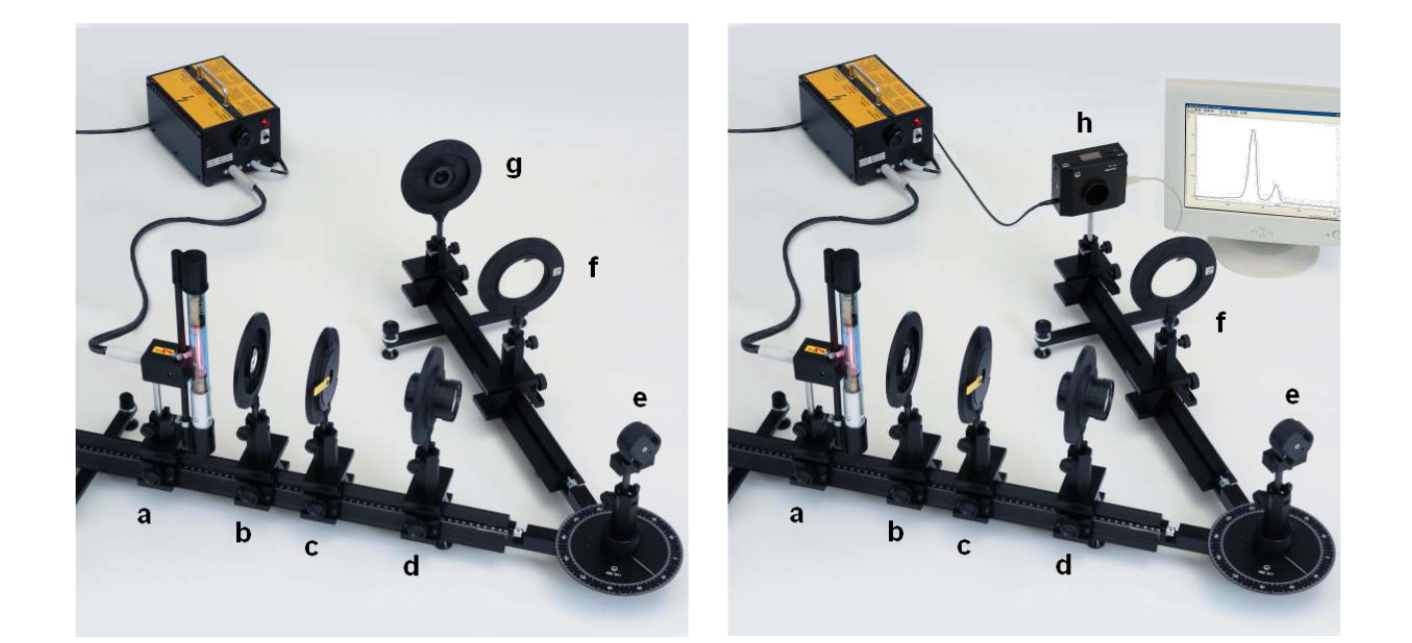
\includegraphics[width=0.7\linewidth]{figs/aufbau_balmer_serie.png}
    \caption{Versuchsaufbau mit Okular(links) und CCD-Kamera(rechts) \ref{prakticum}}
    \label{fig:balmeraufbau}
\end{figure}
Diese ist wie folgt aufgebaut: 

Es befindet sich eine Deuterium Lampe (\textbf{a}), welches durch eine Sammellinese (\textbf{b}) mit Brennweite $f = 50mm$ auf ein Verstellbarer Spalt (\textbf{c}) abgebildet wird. 
Dies soll die Einfallende Lichtstrahl begrenzen. 
Hinter dem Spalt befindet sich ein Projektionsobjektiv (\textbf{d}), mit Brennweite $f = 150mm$. 
Dieses soll genau in Abstand seine Brenweite zu dem Spalt stehen, damit der Lichtstrahl parallel zu dem Holographischen Gitter (\textbf{e}) einfallen. 
Dieses Holographische Gitter ist ein Reflextrionsgitter was sich auf der Drehbaren Säule des Drehgelenksbe befindet und genutzt wird um die Spektrallinien der Lampe aufzuspallten. 
Das reflektierte Licht wird anschliesend mit einer Sammellinse (\textbf{f}) der Brennweite $f=300mm$ auf einem Okular (\textbf{g}) abbildet.
Das Okular kann alternativ mit einer CCD-Kamera (\textbf{h}) für exatere Messungen ersetzt werden.

\section{Durchfühung}

\paragraph{Justierung}\\

Damit die Gitterkonstante bestimmt werden kann, muss von einem bekannten Element die Spektrallinien untersucht werden. 
Dazu wird die Deutrium lampe (Balmer-Lampe) mit einer Quecksilder Lampe (Hg-Lampe) ersätzt. 
Hierzu muss darauf geachtet werden das alle Bauteile des Aufbaus auf der gleichen hohe bleiben, damit es keine veränderungen der optischen achse mit der Balmer-Lampe geben würde.
Es wird nun die Linse \textbf{b} so justiert, das es einen scharfen Lichtfleck von der Lampe auf der Platte abgebildet wird.
Das Projektionsobjektive \textbf{d} wird auf ungefähre Brennweite hinter den Spalt positioniert. 
Es wird nun das Drehgelenk des Gitters (\textbf{e}) auf die 0$^\circ$ position gebracht und das Projektionobjektive so verschoben, dass ein schafes Bild des Spaltes auf dem spalt erkännbar ist, so wird der SPalt im unendlichen abgebildet.
Zuletzt wird die Linse \textbf{f} so justiert, dass im Okular ein scharfes Bild, im Spektrum, zu erkennen ist. Dieses Bild soll eine beliebige Spektrallienie der ersten Ordnung sein.
Nun soll, für den folgenden Versuchsteil, die Winkel des optischen Bank ($\omega_B$) und das Winkel des Gitters ($\omega_G$) abgelesen werden.  
Damit diese werte benutzt werden können, müssen diese in die Relewanten winkel für das Gitter umgerechnet werden, sehe \cref{Gitter Balmer}. 
Mit Hilfe von \cref{Gitter Balmer} können 
\begin{align}
    \alpha &= \omega_G \\  \beta &= \omega_B + \omega_G - 180^\circ 
\end{align}
Dieses Soll nach dem Zurücktausch der Hg-Lampe und der Balmer-Lampe Widerholt werde. 


\paragraph{Bestimmung der Gitterkonstante}\\

Die Gitterkonstent wird mithilfe der Hg-Lampe bestimmt.
Es wird nach dem ersten Spektral linie gesucht, bis dies gefunden ist. 
Hier zu wird die hälichkeit der Spektrallinie über die Spalt aufgedreht, wenn diese nicht sichtbar sind und dann auf etwa 1 Skalen Teil (0,1mm) eingestellt, aber dass die nicht verschindet.
Um zu vergleichen welche Wellenlänge gesehen werden konnte für die auswertung wurde die Hg-Linien von dem Anhang \cref{Hg-Linien} zu nutzen.
Es werden nun $\omega_B$ und $\omega_G$ abgelesen und mit \cref{Hg-Linien} zugeordnet.

\paragraph{Untersuchung der Balmer-Linien}
Nach dem Tauschen der Lampen wird erstmal die Justierung Widerholt. 
Nach der Justierung werden für jede Spektrallinie Widerrum die Winkel $\omega_B$ und $\omega_G$ gemessen und der Abstand der Aufspaltung $d$, der SPektrallinien, abgeschätzt.

\paragraph{Ersätzen Okular mit CCD-Kamera}
Es wird nun das Okular mit einer CCD-Kamera ersätzt, damit eine genauere bestimmung der Spektrallinien stadt finden kann. 
Es wird ein Programm genutzt, welches die Intensität und Pixelkoordinate (Position der Intensität) aufnimmt und gegen einander aufträgt. 
Falls die Intensität zu klein ist, kann im programm die Schaltfläche vergrößert werden.
Das Programm gibt aber einen Winkel aus , den Ausfalls winkel, welches es aus den Pixelkoordinaten entnimmt, mit 
\begin{equation}
    \beta = \arctan(\frac{(1024-p)\cdot0,014mm}{f})
\end{equation}
wobei, $p$ die Pixelkoordinate und $f$ die Brennweite der abbildenden Sammellinse sind.
Diese Linse wird noch verschoben, bis die Darstellung des Programmes Scharf dagestellt werden kann (die Peaks sollen so dünn wie möglich sein).
Da die Intensität sehr sensitive ist, wird mit Hilfe des Programms einen Mittelwerts Bildung der Intensität gemacht. 
Diese Werte werden gespeichert und die Winkel des Gitter aufgenommen. 
Es wird der gleich Vorgang für die weitere Balmer-Linien Verhandet.

\section{Bestimmung der Gitterkonstanten}
Um die Gitterkonstante zu berechnen wird die Gitter gleichung für ein Reflexionsgitter 
\begin{equation}
  g\bigl(\sin\alpha + \sin\beta\bigr) = m\,\lambda
  \quad\Longrightarrow\quad
  g = \frac{m\,\lambda}{\sin\alpha + \sin\beta}
  \label{Gittergleichung}
\end{equation}
genutzt, mit m die Ordnung, $\lambda$ die Wellenlänge, $\alpha$ der Einfall Winkel und $\beta$ der Ausfalls Winkel, mit fehler
\begin{equation}
  \Delta g
  = \sqrt{
    \Bigl(\tfrac{\partial g}{\partial\alpha}\,\Delta\alpha\Bigr)^{2}
   +\Bigl(\tfrac{\partial g}{\partial\beta}\,\Delta\beta\Bigr)^{2}
  }.
  \label{Gitterfgleichung fehler}
\end{equation}
\begin{equation}
  \frac{\partial g}{\partial\theta_m}
  = \frac{m\,\lambda\,\cos\theta_m}{(\sin\theta_m + \sin\beta)^{2}},
  \quad
  \frac{\partial g}{\partial\beta}
  = \frac{m\,\lambda\,\cos\beta}{(\sin\theta_m + \sin\beta)^{2}}.
\end{equation}
\begin{equation}
    \Longrightarrow \Delta g = \sqrt{\Bigl(\tfrac{m\,\lambda\,\cos{\alpha}}{(\sin{\alpha}+\sin{\beta})^2}\,\Delta\alpha\Bigr)^2 + \Bigl(\frac{m\,\lambda\,\cos{\beta}}{(\sin{\alpha} + \sin{\beta})^2}\,\Delta\beta\Bigr)^2}
\end{equation}

Es wird m = 1 gesetzt, da dies die ordnung ist, die untersucht wird.


Dies ausgerechneten Werte befinden sich in \cref{tab:gitterkonstante} mit den Entsprächenden abhängigen werte und dessen fehler.
\begin{table}[htbp]
    \centering
    \begin{tabular}{c|c}
         &  \\
         & 
    \end{tabular}
    \caption{Caption}
    \label{tab:my_label}
\end{table}
Es ist zu bemerken, dass für die roten Spektrallinien für $\omega_B = 145^\circ$ nicht sichtbar waren wurde diese geändert und zur Überprüfung, schon gemessene Spektrallinien nochmals ausfgenommen. 
Zu beachten, ist dass diese Werte nicht genau übereinstimmen, was mit schlechtem abschätzen zu tun haben könnte, da zum Beispiel $61,2^\circ$ und $61,0^\circ$ kaum zu unterscheiden waren.
Mit der Annahme dieses Fehlers sind die Werte angemessen.
Zusätzlich waren manche Linien so blass, das diese kaum erkannt wurden und mehr Linien gesehen wurden. 
Diese wurden aber nicht genommen, da diese sehr schlecht zu sehen waren. 
Um einen festen Wert zu haben um für die Balmer-Linien zu berechnen, wurde der mittelwert von den ausgerechneten Gitterkonstanten genommen mit 

\begin{equation}
  \overline{g}
  = \frac{\sum_{i=1}^{N} \bigl(g_i/\Delta g_i\bigr)}
         {\sum_{i=1}^{N} \bigl(1/\Delta g_i\bigr)},
  \quad
  \Delta\overline{g}
  = \sqrt{\frac{N}{\sum_{i=1}^{N} 1/(\Delta g_i)^{2}}}\,.
\end{equation}

Es ergibt sich nun die Gitterkonstante mit:
\begin{equation}
    \overline{g} = (420.76 \pm 1.51) nm.
    \label{gitterkon}
\end{equation}
Dieser Wert passt nicht zu allen g-Werte, aber mit mehr als $2/3$ und ist somit ein sinvoller Wert. 

\section{Bestimmung der Balmerlinien}

Mit der Gitterkonstante kann nun die Wellenlängen der Balmer-Lampe berechnet werden. 
Dies kann durch die Gittergleichung \ref{Gittergleichung} mit der Ersten Ordnung berechnet werden.
Die dazu gehörige Wellenlängen ist zwischen 388nm und 656nm sichtbar ([Uni Ulm]) und mit den Messung zuzuordnen.
Die Emissionslinien sind dabei die Übergänge von Energieniveau $n > 2 \xrightarrow{} n = 2$ 
Die Photonen die den Übergang beschreiben, kann durch die Rydberg-Formel ([Demtröder Ex3], S.100) 
\begin{equation}
  \frac{1}{\lambda}
  = Ry\Bigl(\tfrac{1}{2^{2}} - \tfrac{1}{n^{2}}\Bigr),
  \quad n=3,4,5,\dots
  \label{Rydberg-Formel}
\end{equation}
gezeigt werden.
Diese wird noch im \cref{Rydberg-konst} bestimmt. 
Es wird nochmals die Winkel für die bestimmten Emissionslinien aufgenommen werden und die Ausgerechneten Werte in \cref{tab: gesehenes deut}, so wie deren Literautrwert aufgelistet. 

Wärend des versuches, wurden nur 3 Emissionslinien gesichtet, dies könnte an dem Fehlenden Abschirmung der Lampe liegen könnte welches durch Reflextion an der linse vor dem Okular, die schwer zu sehenden Emissionslinien, Überleuchtet hat. %Versuche zu sagen, dass wegen das licht der lampe die linie nicht zu sehen ist.
Dieses könnte zu H$_\alpha$, H$_\beta$ und H$_\gamma$ zugeordnet werden.

\begin{table}[htbp]
    \centering
    \begin{tabular}{c|c}
         &  \\
         & 
    \end{tabular}
    \caption{Deuterium}
    \label{tab: gesehenes deut}
\end{table}

Es ist zu sehen, dass die berechneten Wellenlängen nicht mit den Literaturwert übereinstimmt. 
Dies könnte an der näherung der Winkel liegen, da diese zum Beispiel als $55,3^\circ \approx 55,5^\circ$.
Zusätzlich hätten die Fehler auch zu klein Geschetzt werden können.
Obwohl die Werte nicht mit den Fehler mit den Literaturwerte übereinstimmen, sind die Werte genau genug, um die Werte zuzuordnen. 


\subsection{Bestimmung der Isotopieaufspaltung}

Bei der Unteruchung der Emissionslinien der Balmer-linien, wurde gesehen, dass die Emissionslinien eine zweite Emissionslinie existiert.
Der Grund hierfür ist an der Balmer-Lampe. 
Da diese nicht rein aus Deuterium, sonder auch Wasserstoff besteht, im Verhältnis von \approx 1 : 2 ([Praktikum]). 
Dies Weist darauf hin, das die Kern Masse einen Einfluss auf die Energieniveaus hat. 
Aus der Quantenmechanik kann die Rydberg-konsante zusätzlich mit 
\begin{equation}
    Ry = \frac{\mu e^4}{8 c \epsilon_0^2h^3}
\end{equation}
beschrieben werden([Demtröder Ex3], S.101). Dabei ist zu beachten, dass dieser wert von der Reduzierten Masse abhängt.
Durch 
\begin{equation}
    \mu = \frac{m_e \cdot m_K}{m_e + m_K} = \frac{m_e}{1+\frac{m_e}{m_K}}
\end{equation}
mit $m_e$ die Elektronen Masse und die Kernmasse $m_K$.
Somit kann ein fester Rydbergkonstante ($Ry_\infty$) bestimmt werden: 
\begin{equation}
    Ry = \frac{1}{1+\frac{m_e}{m_K}}\cdot \frac{\mu m_e e^4}{8c \epsilon_0^2h^3} = \frac{1}{1 + \frac{m_e}{m_K}}\cdot Ry_\infty
\end{equation}
Da das Deuterium einen extra Neutron hat ist dieses Schwärer, somit ist die Ry kleiner und so auch proportional die Wellenlänge. 
Dieses wurde auch für größere Wellenlänge deutlicher sichtbar.
Diese Aufspeltung wird als Isotopieaufspaltung bezeichnet, wobei es sich in diesem fall über ein Masseneffekt der Isotopiaufspaltung handelt.

Mit der Skala in dem Okular kann die Größe d der Isotopieaufspaltung für die Emissionslinien geschätzt werden. 
Diese befinden sich in \cref{tab:Isotopie}.

Dies kann durch die \cref{Gittergleichung}
\begin{equation}
  \lambda = g\,(\sin\alpha + \sin\beta),
  \quad
\frac{\Delta\lambda}{\Delta\beta} \approx 
  \frac{\partial\lambda}{\partial\beta} = g\,\cos\beta,
  \quad
  \Delta\beta \approx \frac{d}{f},
\end{equation}
und mit der Brennweite der Abbildungslinse kann sich der Winkel $\Delta\beta$ durch 
\begin{equation}
    \Delta\beta = \arctan\Bigl(\frac{d}{f}\Bigr) \approx \frac{d}{f} \quad \text{für } d \ll f
\end{equation}
berechnen lassen.

Diese Werte sind aber nicht genau, da diese aufspaltung sehr schwer zu sehen war und nur mit mühe versucht abzuschätzen.

Die CCD-Kamera hat dieses Problem aber nicht und kann genauer die Isotopieaufspaltung Messen.

Die Gemessenen Intensitäten Bilden Peaks die in \cref{fig:H_a},\ref{H_b} und \ref{H_g} dargestellt sind. 
Hierbei sind mehrere Peaks zu erkennen und können durch folgende Gauß-Peak Funktion 
\begin{equation}
    I(\beta) = \sum_i^2 A_i \cdot \exp{\Bigl(-\frac{\beta-\mu_i}{2\sigma_i}}\Bigr) +b
\end{equation}
berechent werden, mit b, dem Offset und dem Winkel $\beta$. 
